\documentclass{article}
\usepackage{hyperref}
\usepackage[latin1]{inputenc}
\parindent=0pt
\parskip=2pt
\usepackage{indentfirst}
\usepackage[top=2cm, bottom=2cm, left=3cm, right=2cm]{geometry}
\usepackage{xcolor}
\usepackage{graphicx}
\usepackage{tabularx}

\title{Linguagens de Programa��o - Trabalho 1}
\author{Ewerton Vasconcelos da Silva
        \and 
        Gabriel Silva Lopes }
\date{Abril de 2017}





\begin{document}

\begin{tabularx}{\linewidth}{c X}
\parbox[c]{3cm}{
\includegraphics[width=\linewidth]{UFRJ}} &
	\begin{center}
		\textsc{Universidade Federal do Rio de Janeiro\\
			Escola Polit�cnica \\
			Departamento de Eletr�nica e de Computa��o
		}
	\end{center}
\end{tabularx}

\begin{center}
\LARGE
		\textbf{Linguagens de Programa��o}\\
\Large
		\textbf{Trabalho 1}\\
		Ewerton Vasconcelos e Gabriel Lopes
\end{center}

\section{Introdu��o}
 O algoritmo conhecido como Comb Sort fora criado por Wlodzimierz Dobosiewicz em 1980, por�m somente em 1991 foi popularmente divulgado por Stephen Lacey e Richard Box 
 
 
\section{A defini��o do Problema}
O Comb Sort � baseado no bubble Sort, por�m alguns conceitos na implementa��o o torna mais eficiente. enquanto o Blubble Sort realiza varreduras comparando pares de elementos

\begin{figure}[htbp!] \begin{center}
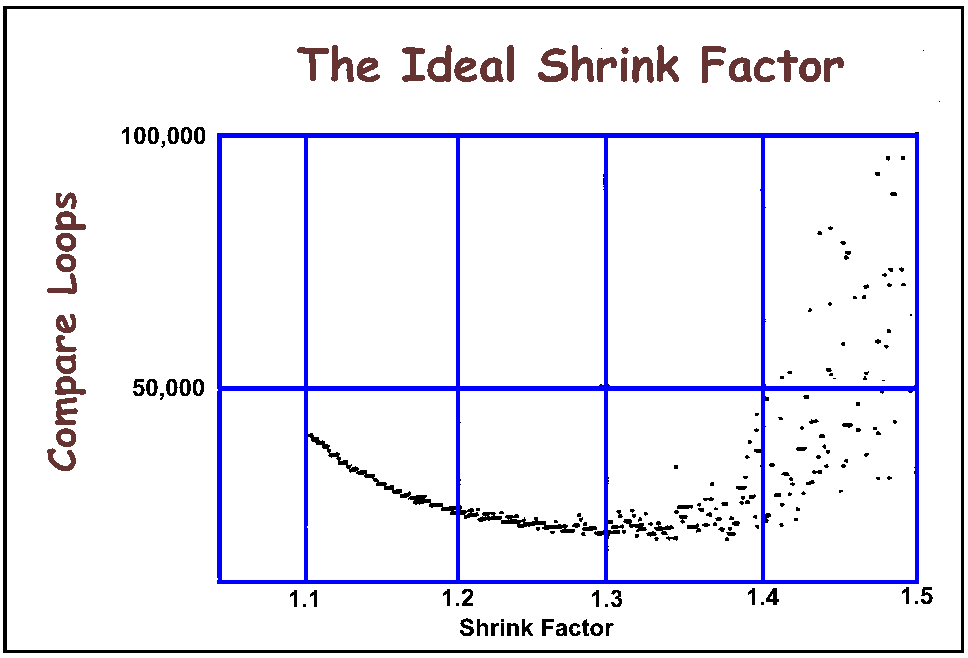
\includegraphics[width=0.6\linewidth]{fig1}
\caption{Gr�fico dos Testes para determina��o do fator encolhimento. Gr�fico Original do Artigo da Revista BYTE}
\end{center} \end{figure}


\section{Inputs e Outputs do Software}
Para o Comb Sort Temos as Seguintes complexidades Assint�ticas.

\section{O Papel de Cada Software}
Para o Comb Sort Temos as Seguintes complexidades Assint�ticas.
\begin{itemize}
\item C++: \\
Como Temos 2 loop While concatenados, no pior caso, ambos os loops s�o executados $n$ vezes.
\item Perl: \\
Como Temos 2 loop While concatenados, no pior caso, ambos os loops s�o executados $n$ vezes.
\end{itemize}

\section{O Software em C++}
O Comb Sort � baseado no bubble Sort, por�m alguns conceitos na implementa��o o torna mais eficiente. enquanto o Blubble Sort realiza varreduras comparando pares de elementos

\section{O Software em Perl}
O Comb Sort � baseado no bubble Sort, por�m alguns conceitos na implementa��o o torna mais eficiente. enquanto o Blubble Sort realiza varreduras comparando pares de elementos

\section{Conclus�o}
O algoritmo Comb Sort se mostrou muito eficiente, devido sua baixa complexidade para alguns casos, e complexidade aceit�vel em casos
m�dios. Outro ponto interessante al�m da sua boa complexidade assint�tica, � sua f�cil implementa��o. Portanto, o Comb Sort se mostrou interessante para aplica��es corriqueiras. 




\end{document}
